\subsubsection{Scheduling Energy-Aware in Ambienti FaaS Federati ed Eterogenei}
\label{subsubsec:greenfaas}

In ambienti FaaS federati o multi-sito, la decisione di \emph{placement}
non dipende soltanto dall'efficienza del nodo di calcolo, ma anche dal
costo energetico necessario a rendere disponibili i dati di input nel
sito selezionato. In questi scenari, risorse eterogenee e
geograficamente distribuite — tra cui cluster HPC, workstation e
infrastrutture cloud — presentano profili energetici differenti, e le
funzioni possono operare su dataset residenti in domini amministrativi
distinti. Ne consegue che l'allocazione ottimale deve considerare
congiuntamente il costo di \emph{computation} e di \emph{communication},
evitando scelte che riducono il consumo di esecuzione introducendo al
contempo overhead energetici significativi dovuti alla movimentazione
dei dati.

In questo contesto si colloca GreenFaaS~\cite{greenfaas}, un framework
progettato per orchestrare invocazioni FaaS in ambienti distribuiti,
integrando nella decisione di scheduling una stima esplicita del costo
energetico dei trasferimenti. Come mostrato in
Figura~\ref{fig:greenfaas_arch}, l'architettura si articola in tre
componenti principali: un modulo di \emph{Resource Monitoring}, un
\emph{Transfers Manager} e uno \emph{Scheduler}.

\begin{figure}[ht]
\centering
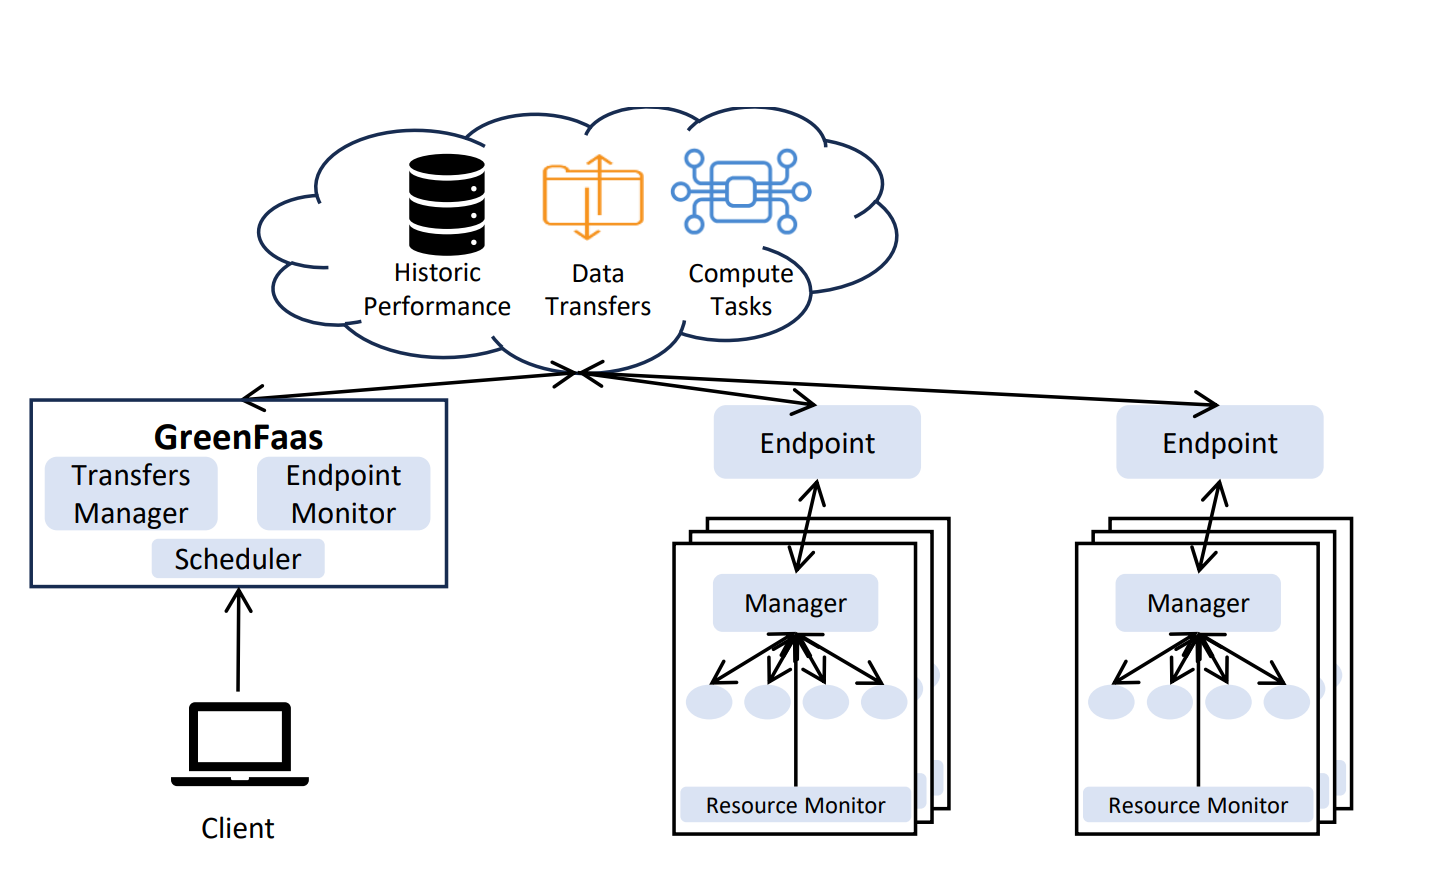
\includegraphics[width=0.9\textwidth]{figures/GreenFaas.png}
\caption{Architettura di alto livello di GreenFaaS: monitoraggio degli
endpoint, stima del costo energetico dei trasferimenti e scheduling
energy-aware per l'allocazione dei task in ambienti federati eterogenei.}
\label{fig:greenfaas_arch}
\end{figure}

Il modulo di monitoraggio raccoglie a runtime metriche energetiche e
prestazionali dei nodi, sfruttando interfacce hardware — tra cui RAPL
per CPU e NVML per GPU — per derivare stime di potenza e caratterizzare
il comportamento energetico delle risorse disponibili. Tali misure
consentono di stimare il costo di esecuzione su piattaforme eterogenee,
riducendo la dipendenza da proxy indiretti quali il solo tempo di
esecuzione.

Il \emph{Transfers Manager} modella il contributo energetico associato
alla movimentazione dei dati tra siti. Quando l'input risiede in un
dominio diverso da quello candidato all'esecuzione, il trasferimento
introduce un costo legato alla trasmissione in rete e alle operazioni
di I/O agli estremi della comunicazione. GreenFaaS stima tale costo in
funzione della dimensione dei dati e delle caratteristiche del
collegamento, consentendo di quantificare l'impatto energetico della
scelta del sito anche nei casi in cui il nodo remoto risulti
computazionalmente più efficiente.

Sulla base di queste informazioni, lo \emph{Scheduler} effettua una
selezione multi-criterio che integra il consumo energetico previsto per
l'esecuzione sul nodo candidato e il costo energetico dei trasferimenti
eventualmente necessari, affiancando a tali grandezze una stima del
tempo di completamento. Il peso relativo delle componenti è
configurabile, consentendo di modulare il compromesso tra efficienza
energetica e prestazioni in funzione degli obiettivi applicativi. Per
mantenere la reattività in presenza di carichi dinamici e
infrastrutture di grandi dimensioni, il framework adotta strategie
euristiche che evitano un'ottimizzazione globale onerosa. Nei contesti
in cui il consumo in stato di inattività risulti significativo, sono
inoltre previsti meccanismi di raggruppamento di task con profili simili,
con l'obiettivo di ammortizzare il costo fisso di attivazione su
esecuzioni consecutive.

Nel complesso, GreenFaaS amplia la nozione di consapevolezza energetica
nello scheduling FaaS oltre la sola scelta del nodo computazionale,
estendendola al costo di comunicazione tra siti. Questo contributo
è particolarmente rilevante in architetture federali con forte
dispersione geografica, dove i trasferimenti dati possono dominare il
bilancio energetico complessivo e rendere subottimali le scelte basate
esclusivamente sull'efficienza di calcolo locale.